\chapter{Measurement of Directional Characteristics II}\label{ax:directional_2}
This appendix serves as a protocol to a series of measurements conducted on the 2\textsuperscript{nd} of March 2018 in the large anechoic chamber (B4-111) at the acoustical lab of Aalborg University at Fredrik Bajers Vej 7.\\
The goal of these measurements was to quantify the directional characteristics of the loudspeakers that will be used in the loudspeaker array. The results are useful to show, what assumptions can be made when the speaker array is set up and where the position of the acoustic center is in relation to the cabinet. They will also serve as a baseline to which the directional characteristics of the speaker array can be compared. Furthermore, more experience can be gained regarding the practical aspects of measurement.

\section*{Measuring Equipment and Materials}
The following measuring equipment was used:
\begin{itemize}[noitemsep]
\item Microphone \gls{bandk} 4144
\begin{itemize}[noitemsep]
\item AAU-number: 06552
\item Serial number: 297090
\end{itemize}
\item Preamplifier GRAS 26AK
\begin{itemize}[noitemsep]
\item AAU-number: 56525
\item Serial number: 32811
\end{itemize}
\item Power supply \gls{bandk} 2804
\begin{itemize}
\item AAU-number: 06998
\item Serial number: 455309
\end{itemize}
\item Calibrator \gls{bandk}\ 4231
\begin{itemize}[noitemsep]
\item AAU-number: 33691
\item Serial number: 2115338
\end{itemize}
\item Power Amplifier Pioneer A-616
\begin{itemize}[noitemsep]
\item AAU-number: 08249
\item Serial number: HJ9404841S
\end{itemize}
\item Sound card RME Fireface UCX
\begin{itemize}[noitemsep]
\item AAU-number: 108230
\item Serial number: 23811948
\end{itemize}
\item Turntable: Outline ET 250-3D
\begin{itemize}
\item Serial number: REIBO012
\end{itemize}
\item MATLAB r2017b on OSX 10.11.6
\item Loudspeaker SEAS 33 F-WKA
\end{itemize}

The following material was used:
\begin{itemize}[noitemsep]
%\item \SI{1/2}{\inch} to \SI{1}{\inch} preamp adapter
\item Microphone clip
\item Microphone stand
\item LEMU cable
\item XLR cable
\item Ethernet cable
\item Loudspeaker stand
\item Loudspeaker cabinet, plywood, outside dimensions: (400x400x400)\SI{}{\milli\meter}, wall~thickness:~\SI{20}{\milli\meter}
\item Speaker mount for turntable
\begin{itemize}[noitemsep]
\item Circular \gls{mdf} cutout, thickness: \SI{12}{\milli\meter}, {\(\varnothing\)~:~\SI{800}{\milli\meter}}
\item Top plate (\gls{mdf}), thickness: \SI{12}{\milli\meter}, surface : (400x400)\SI{}{\milli\meter}
\item 3 battens, (40x40x900)\SI{}{\milli\meter}
\item 3 aluminium brackets
\item 8 bolts M8x30, associated washers
\item miscellaneous woodscrews

\end{itemize}
\end{itemize}

\section*{Setup}
A sketch of the measurement setup can be found in \autoref{fig:measurement_setup}. A picture is given in \autoref{fig:setup_03_02}. \\
According to the findings from \autoref{ax:directional_1} the cabinet had to be backwards from the center of the turntable in order to get the acoustic center of the loudspeaker on the rotational axis. This put up a considerable challenge on the mechanical side.
The 13'' loudspeaker and the cabinet add up to a comparatively large mass. The further they are moved away from the center of the turntable, the more significant are the issues arise, caused by leverage and inertia. This also manifests in \autoref{sec:03_02_results}.
In order to place the the speaker away from the center of the turntable, a circular plane with a diameter of \SI{800}{\milli\meter} was cut out of \SI{12}{\milli\meter} thick \gls{mdf} board and mounted to the turntable. In order to minimize the influence of reflections from the \gls{mdf} board on the measurement, the speaker was raised by \SI{1}{\meter} utilizing wooden pillars. The board on which the loudspeaker rests has the same (400x400)\SI{}{\milli\meter} size as the bottom side of the cabinet. This allows for minor positioning adjustments.\\
Both the microphone and the loudspeaker had a vertical distance of \SI{1.32}{\meter} to the metal grids on which they were standing. The microphone was placed on the main axis of the loudspeaker. The horizontal distance between the front plane of the speaker cabinet and the microphone membrane was \(d=\)\SI{2.74}{\meter}.
The gain potentiometer of the power amplifier was set to \SI{-16}{\decibel} and the \texttt{playgain}-parameter (see XXXXXXX) was set to \SI{-18}{\decibel}.

\begin{figure}[htbp]
	\centering
	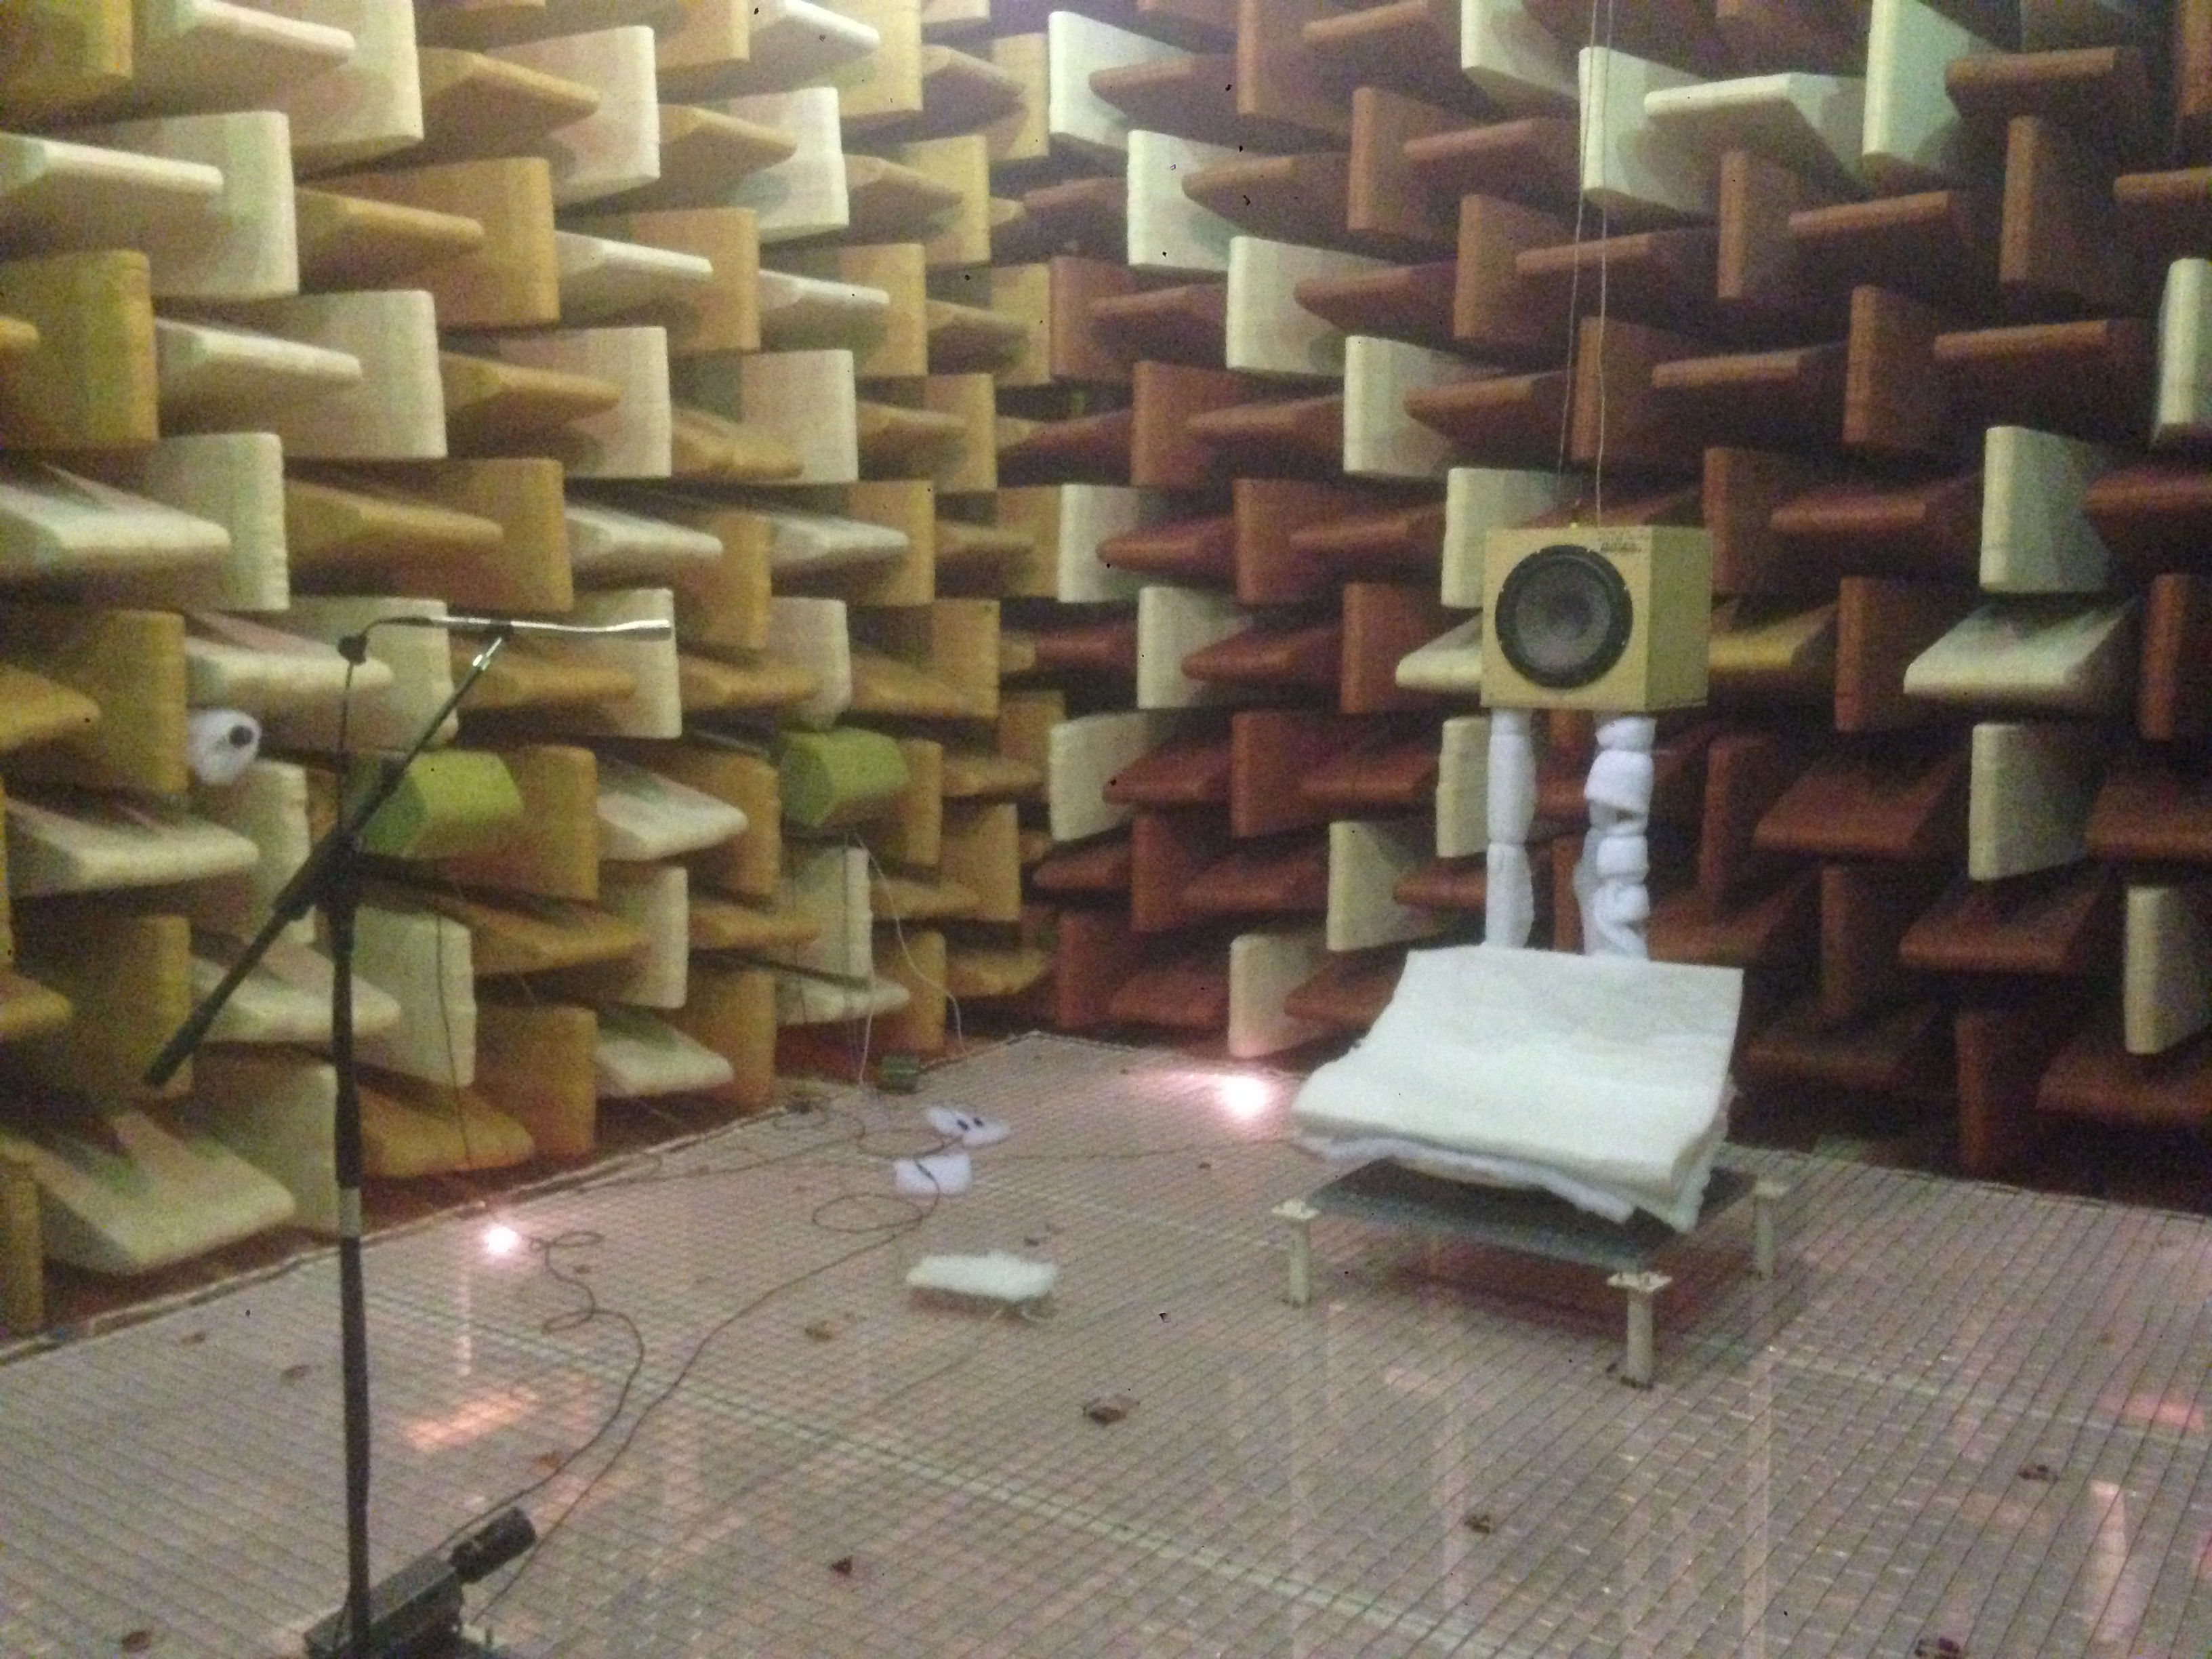
\includegraphics[width=0.7\textwidth]{03_02_setup.JPG}
	\caption{Measurement setup}
		\label{fig:setup_03_02}
\end{figure}

\section*{Results}\label{sec:03_02_results}
The polar response is represented in \autoref{fig:03_02_m1_pressure} and \autoref{fig:03_02_m1_phase}. The front plane of the cabinet had a distance of \SI{115}{\milli\meter} to the rotational axis of the turntable.\\
\autoref{fig:03_02_m1_pressure} shows the normed sound pressure level  along the circumference at different frequencies. The level difference  between the \SI{0}{\degree} and the \SI{180}{\degree} data point is approx. \SI{0.4}{\decibel} at the frequencies of \SI{60}{\hertz} and \SI{100}{\hertz}. Until \SI{150}{\hertz} the graphs have an almost circular shape, that is slightly offset towards the \SI{0}{\degree}. The remaining graphs towards higher frequencies tend to have a shape that is different from that of a circle.
\begin{figure}[htbp]
	\centering
	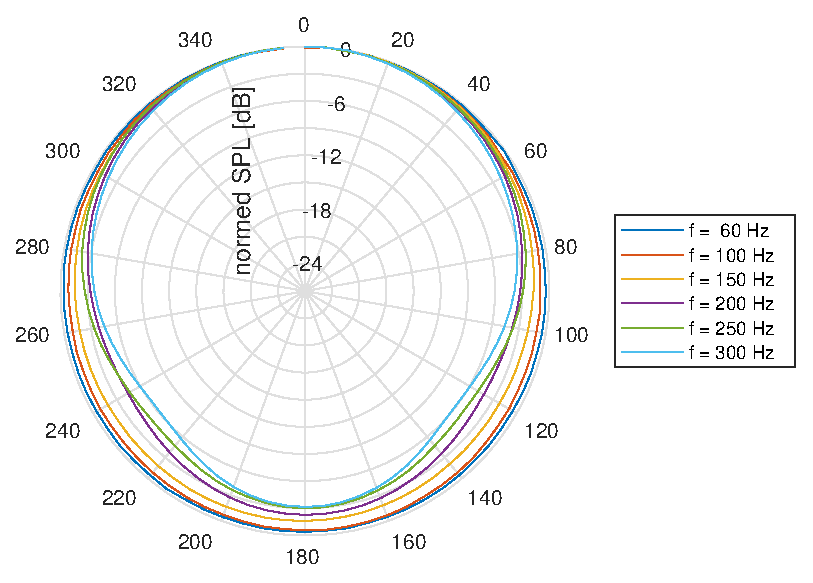
\includegraphics[width=0.7\textwidth]{03_02_meas1_pressure.eps}
	\caption{Normed \gls{spl}, measured at a distance \(d=\)\SI{2.74}{\meter}}
		\label{fig:03_02_m1_pressure}
\end{figure}
\autoref{fig:03_02_m1_phase} visualizes the phase in an angular range from \SI{-180}{\degree} to \SI{180}{\degree} phase angle. Values outside of this range have been shifted by integer multiples of \SI{360}{\degree}. Similar to \autoref{fig:03_02_m1_pressure}, the graphs up to a  frequency of \SI{150}{\hertz} have a near-circular shape. The circles are also slightly offset towards the \SI{0}{\degree} direction. At higher frequencies, the shape gradually changes towards something closer to a cardiod.
As indicated  by the non-concentric graphs and the calculation in \autoref{sec:ac_center}, the acoustic center of the loudspeaker still seems to be in front of the rotational axis by some margin. To move it back the calculated distance, changes to the mechanical support system have to be implemented and another measurement has to be conducted.
\begin{figure}[htbp]
	\centering
	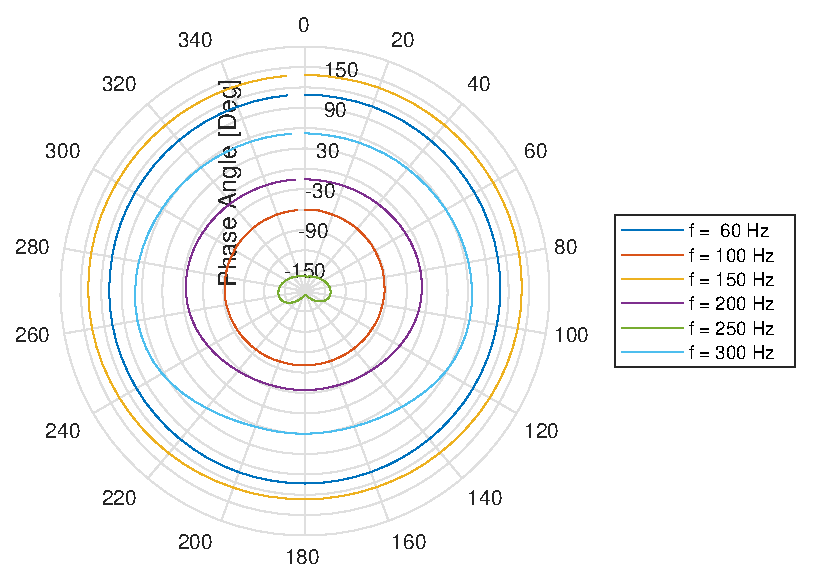
\includegraphics[width=0.7\textwidth]{03_02_meas1_phase.eps}
	\caption{Phase (uncalibrated), measured at a distance \(d=\)\SI{0.75}{\meter}}
		\label{fig:03_02_m1_phase}
\end{figure}


